%%
%% Interaction 2024 Technical Report Submission
%% V1.0 (2023/12/22)
%% 

\documentclass[submit,techrep,english]{ipsj}


\usepackage{graphicx}
\usepackage{latexsym}
\usepackage{url}


\def\Underline{\setbox0\hbox\bgroup\let\\\endUnderline}
\def\endUnderline{\vphantom{y}\egroup\smash{\underline{\box0}}\\}
\def\|{\verb|}

\setcounter{volume}{64}%vol53=2012
\setcounter{number}{10}
\setcounter{page}{1}

% インタラクション特有の設定。印刷工程で柱・ノンブルの埋め込みを行う。
\makeatletter
\pagestyle{empty}
\def\@oddhead{}%
\def\@evenhead{}%
\def\ps@IPSJTITLEheadings{}
\makeatother


\begin{document}


\title{MyStoryKnight: A Character-drawing Driven Storytelling System Using LLM Hallucinations}

\affiliate{LU}{Lund University}
\affiliate{TUD}{Technical University of Denmark}
\affiliate{HRI}{Honda Research Institute Japan}
\affiliate{UTokyo}{The University of Tokyo}
\paffiliate{PUTokyo}{The University of Tokyo}

\author{Yotam Sechayk}{UTokyo}[sechayk-yotam@g.ecc.u-tokyo.ac.jp]
\author{Gabriela A. Penarska}{TUD,PUTokyo}[gabriela-penarska@g.ecc.u-tokyo.ac.jp]
\author{Isa A. Randsalu}{LU,PUTokyo}[randsalu-isa071@g.ecc.u-tokyo.ac.jp]
\author{Christian Arzate Cruz}{HRI}[]

\author{Takeo Igarashi}{UTokyo}[]


\begin{abstract}
    Storytelling is a valuable tradition that plays a crucial role in child development, fostering creativity and a sense of agency. However, many children often consume stories passively, missing out on the opportunity to participate in the creative process. To address this, we propose a storytelling system that creates adventure-type stories with multiple branches that users can explore. We generate these interactive stories using a character drawing as input, with visual features extraction using GPT-4. By leveraging LLM hallucinations, we generate interactive stories using user feedback as a prompt. Finally, we refine the quality of the generated story through a complexity analysis algorithm. We believe that the use of a drawing as input further improves the engagement in the story and characters.
\end{abstract}

\maketitle

%1
\section{Introduction}
\label{sec:introduction}
Creativity is increasingly recognized as a crucial aspect of the modern working environment. In the context of child development, creativity plays a pivotal role in fostering learning and growth \cite{1:ElgarfP22}, which extends to adulthood. As a result, there has been a growing interest in leveraging creative artificial intelligence (AI) and exploring the use of AI agents to stimulate children's creativity. Previous research has demonstrated the positive effects of incorporating AI agents with creative abilities in enhancing children's creative thinking. Additionally, the use of storytelling robots and virtual characters as interactive tools has gained traction in recent years \cite{7:SunLLL17}. In this paper, we propose \textit{MyStoryKnight}, an interactive AI tool for generating stories.

Our proposed system is intended to promote children's creativity through storytelling, a popular activity for entertaining and bonding \cite{7:SunLLL17}. Both storymaking and storytelling contribute to the development of verbal and social skills \cite{9:RyokaiC99,5:CurrinDPCFGH23}, such as broadening the vocanulary and improving  narrative comprehension. Besides, creating fictional worlds and characters helps children improve their language skills, both in comprehension and usage \cite{13:abs-2011-04242}. In \textit{MyStoryKnight}, users, together with an AI, co-create stories with multiple explorable branches.

Despite all the benefits of practicing storytelling, many children do not have the opportunity to engage in interactive storytelling. \textit{MyStoryKnight} addresses this problem by generating an adventure-type story through LLM hallucinations. Figure \ref{fig:system-overview}  shows an overview of our system. Our system uses drawings of characters as input, and generates an unfolding story that the user can navigate through based on their choices. Using a complexity analysis algorithm, we guide the LLM hallucinations to generate a coherent and consistent story. Resulting in a story that is both engaging and easy to follow.

\begin{figure*}[t]
    \centering
    
\includegraphics[width=0.9\textwidth]{figures/2400x600px.png}
    \caption{MyStoryKnight system overview.}
    \label{fig:system-overview}
\end{figure*}

Our contributions are:
\begin{itemize}
    \item Storytelling system that uses the character drawing as a basis for the story.
    \item LLM hallucinations to generate an adventure-type story with user navigation.
    \item Complexity analysis of story generation for coherency and consistency.
\end{itemize}


%2
\section{Related Work}
\label{sec:related-work}

\subsection{Interactive Storytelling}
Interactive storytelling is a form of storytelling in which the audience is an active participant \cite{14:WangRCRMB22}. Interactive storytelling has been shown to be an effective way of building and strengthening relationships \cite{15:SchlauchSG22}, also playing an important role in parent-child bonding \cite{12:ZhangXWYRWYWL22}. Interactive stories stimulate thinking and imagination \cite{11:LimaGV20}, and help children make sense of their world through shared experiences \cite{9:RyokaiC99}.

Prior work has explored physical interactivity through the use of tangible objects \cite{9:RyokaiC99} to create stories, and physical gestures to control characters \cite{2:LiuLWCS12} or generate stories \cite{3:ZhaoB23}. Other studies have explored the use of sketches to influence character behavior and plot development \cite{11:LimaGV20}. However, these studies have not explored the use of character drawings as the driving force behind the story.

\subsection{AI Storytelling}
AI usage has been experiencing a surge in popularity in recent years, with many applications in the creative arts. Generative AI especially has the potential to contribute to creative processes \cite{6:TholanderJ23}. One such creative process could be storytelling. Prior work has explored how generative AI can be used to create stories \cite{13:abs-2011-04242}, and even collaborate in story generation with humans \cite{8:ShakeriND21}. Other studies explored how generative AI can be used to expand existing story worlds \cite{10:ChopraVSS21}, or generate multi-modal storytelling experiences \cite{4:HanC23}. However, while consistency and coherency are essential in storytelling, they are often overlooked in AI-generated stories.

\subsection{Storytelling with Children}
Children oriented storytelling has been explored widely in the past. Prior work has explored the use of robots as storytelling companions \cite{7:SunLLL17}, and the use of virtual characters to promote collaboreation \cite{2:LiuLWCS12}. Other studies have explored the use of AI agents to stimulate children's creativity \cite{1:ElgarfP22}. Other studies have shown how AI can support parent-child bonding \cite{12:ZhangXWYRWYWL22}, and encourage physical interaction and play \cite{3:ZhaoB23}.
However, utilizing hallucinations to generate stories has not been explored in the context of user-agency for storytelling with children.

%3
\section{System Overview}
\label{sec:system-overview}
To address these issues, we designed \textbf{MyStoryKnight}, an interactive storytelling that uses drawings as input and utilizes LLM hallucinations to generate a branching story. Agency is a critical factor in interactive storytelling \cite{11:LimaGV20}, as it promotes engagement and immersion \cite{12:ZhangXWYRWYWL22}. Our system supports user agency by allowing users to navigate the story through their choices. Additionally, we use a complexity analysis algorithm to guide the LLM hallucinations to generate a coherent and consistent story, fitting for children's comprehension.

\subsection{System Architecture}
\label{subsec:system-architecture}
The system architecture is shown in Figure \ref{fig:system-architecture}. The system consists of three main components:
\begin{enumerate}
    \item \textbf{Drawing Analysis}: Extracting visual features from the user's drawing. The visual features are used as a prompt for the LLM to hallucinate a character description and a background story.
    \item \textbf{Story Generator}: Story is generated based on user selection on a set of actions. LLM hallucinations are used to generate the story and actions.
    \item \textbf{Complexity Analysis}: Natural language processing (NLP) techniques are used to analyze the story's coherency and consistency. The results are used to guide the LLM hallucinations.
\end{enumerate}
To achieve out goals, we utilize GPT-4 \cite{17:abs-2303-08774} for drawing analysis and story generation. Additionally, we use spacy \cite{18:spacy} in addition to GPT-4 for complexity analysis. The system is implemented with Django, a Python web framework \cite{19:django}, and React, a JavaScript library for building user interfaces \cite{20:react}.

\begin{figure}[t]
    \centering
    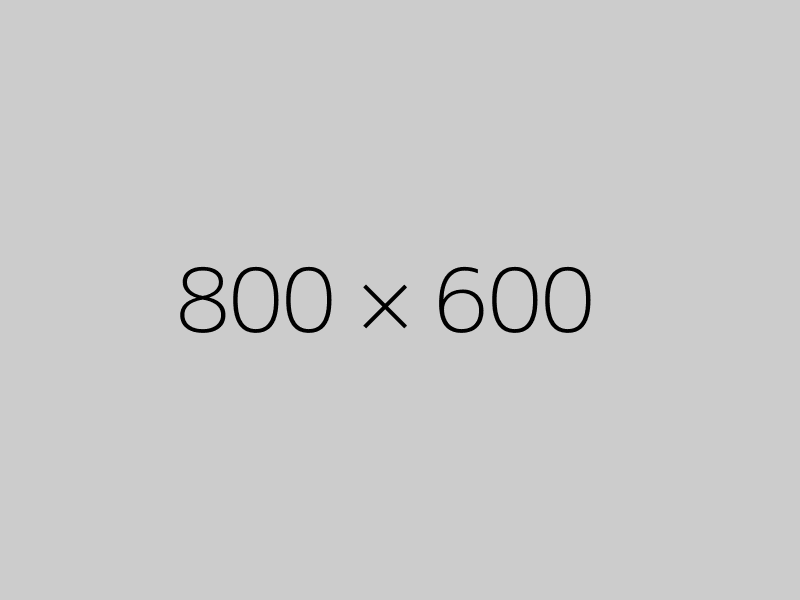
\includegraphics[width=0.45\textwidth]{figures/800x600px.png}
    \caption{System architecture.}
    \label{fig:system-architecture}
\end{figure}

\section{User Interface}
\label{sec:user-interface}
The user interface is shown in Figure \ref{fig:user-interface}. There are three

\begin{figure}[t]
    \centering
    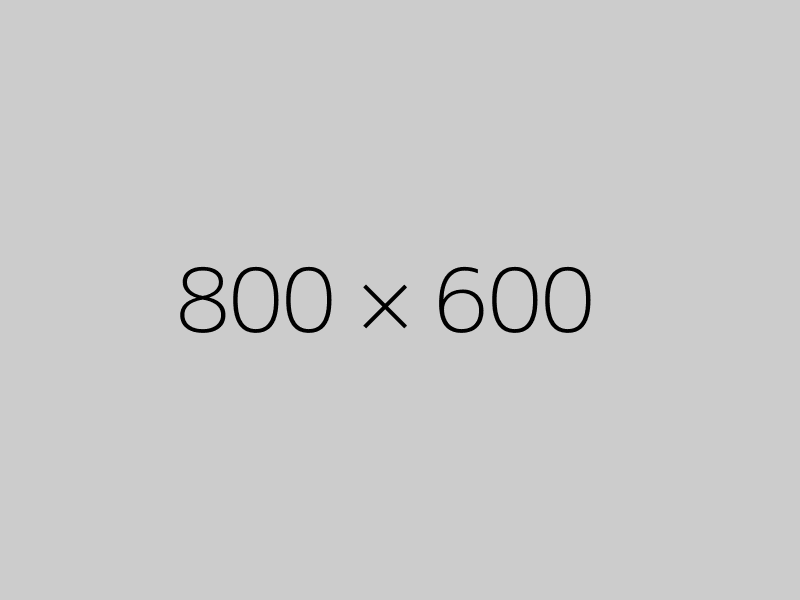
\includegraphics[width=0.45\textwidth]{figures/800x600px.png}
    \caption{User interface.}
    \label{fig:user-interface}
\end{figure}

\subsection{Interaction Flow}
\label{subsec:interaction-flow}

%4
\section{Conclusion}

% Acknowledgment
\begin{acknowledgment}
    Test.
\end{acknowledgment}

% Bibliography
\bibliographystyle{ipsjsort-e}
\bibliography{references}

% Appendix
\appendix

\end{document}
